\begin{figure}[t]
\centering
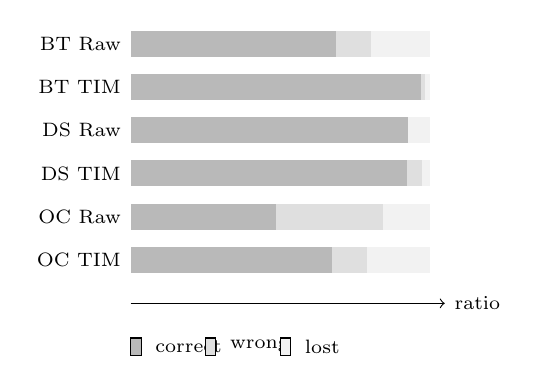
\begin{tikzpicture}[
    x=38mm,
    y=5.5mm,
    font=\scriptsize
]
\draw[->] (0,0) -- (1.05,0) node[right] {ratio};

\node[anchor=east] at (0,6) {BT Raw};
\fill[gray!55] (0,5.7) rectangle (0.687,6.3);
\fill[gray!25] (0.687,5.7) rectangle (0.802,6.3);
\fill[gray!10] (0.802,5.7) rectangle (1.000,6.3);

\node[anchor=east] at (0,5) {BT TIM};
\fill[gray!55] (0,4.7) rectangle (0.969,5.3);
\fill[gray!25] (0.969,4.7) rectangle (0.984,5.3);
\fill[gray!10] (0.984,4.7) rectangle (1.000,5.3);

\node[anchor=east] at (0,4) {DS Raw};
\fill[gray!55] (0,3.7) rectangle (0.928,4.3);
\fill[gray!25] (0.928,3.7) rectangle (0.928,4.3);
\fill[gray!10] (0.928,3.7) rectangle (1.000,4.3);

\node[anchor=east] at (0,3) {DS TIM};
\fill[gray!55] (0,2.7) rectangle (0.923,3.3);
\fill[gray!25] (0.923,2.7) rectangle (0.974,3.3);
\fill[gray!10] (0.974,2.7) rectangle (1.000,3.3);

\node[anchor=east] at (0,2) {OC Raw};
\fill[gray!55] (0,1.7) rectangle (0.487,2.3);
\fill[gray!25] (0.487,1.7) rectangle (0.843,2.3);
\fill[gray!10] (0.843,1.7) rectangle (1.000,2.3);

\node[anchor=east] at (0,1) {OC TIM};
\fill[gray!55] (0,0.7) rectangle (0.672,1.3);
\fill[gray!25] (0.672,0.7) rectangle (0.791,1.3);
\fill[gray!10] (0.791,0.7) rectangle (1.000,1.3);

\node[anchor=west] at (0.05,-1.0) {correct};
\draw[fill=gray!55] (0,-1.2) rectangle (0.035,-0.8);
\node[anchor=west] at (0.30,-1.0) {wrong};
\draw[fill=gray!25] (0.25,-1.2) rectangle (0.285,-0.8);
\node[anchor=west] at (0.55,-1.0) {lost};
\draw[fill=gray!10] (0.50,-1.2) rectangle (0.535,-0.8);
\end{tikzpicture}
\caption{Stacked selected-target correctness ratios. TIM-MARS strongly reduces wrong-target output for ByteTrack and OCSORT.}
\label{fig:result_ratios}
\end{figure}
